\documentclass[a4paper,10pt,twocolumn]{ltjarticle}
\usepackage{kaitoushu}

\pgfplotsset{
  myaxis/.style={
    axis lines=middle,
    xlabel={$x$}, ylabel={$y$},
    every axis x label/.style={at={(ticklabel* cs:1)},anchor=west},
    every axis y label/.style={at={(ticklabel* cs:1)},anchor=south},
    tick label style={font=\scriptsize},
    label style={font=\small},
    width=5.5cm, height=5cm,
    grid=none,
    samples=200,
  }
}

\begin{document}

\problemrange{4章：指数関数と対数関数 — 練習問題1・A (p.110)}



\mondai{1}{次の式を計算せよ．ただし，$a>0$ とする．}
\kotae{
有理指数に統一して指数法則で計算する．

\textbf{(1)} $\sqrt[4]{16a^{8}}=(16a^{8})^{1/4}=2^{4\cdot1/4}\cdot a^{8/4}=2a^{2}$

\textbf{(2)} $\left(\sqrt[6]{a^{-2}}\right)^{3}=\left(a^{-2/6}\right)^{3}=a^{-1}=\dfrac{1}{a}$

\textbf{(3)} $\left(\sqrt[4]{a^{3}}\right)^{2}\times\sqrt{a}=a^{3/2}\cdot a^{1/2}=a^{2}$

\textbf{(4)} $\sqrt[3]{a^{2}}\div\sqrt[4]{a}=a^{2/3-1/4}=a^{8/12-3/12}=a^{5/12}$
}

\mondai{2}{次の数を大きいものから順に並べよ．}
\kotae{
\textbf{(1)} $\sqrt[4]{9},\;3^{-1/2},\;1,\;\sqrt[3]{9},\;9^{-1/3}$

底を $9$ に揃える：
\[
\sqrt[4]{9}=9^{1/4},\;3^{-1/2}=9^{-1/4},\;\sqrt[3]{9}=9^{1/3},\;1=9^{0}
\]

指数の大小：$\dfrac{1}{3}>\dfrac{1}{4}>0>-\dfrac{1}{4}>-\dfrac{1}{3}$．底 $9>1$ は単調増加．

$\therefore \sqrt[3]{9}>\sqrt[4]{9}>1>3^{-1/2}>9^{-1/3}$

\textbf{(2)} $1,\;0.3^{-2},\;\dfrac{1}{0.3},\;\sqrt{0.3},\;\sqrt[3]{0.3}$

底を $0.3$ に揃える：
\[
0.3^{-2},\;0.3^{-1},\;0.3^{0},\;0.3^{1/2},\;0.3^{1/3}
\]

指数の大小：$-2<-1<0<\dfrac{1}{3}<\dfrac{1}{2}$．底 $0.3<1$ なので値は逆順：

$\therefore 0.3^{-2}>\dfrac{1}{0.3}>1>\sqrt[3]{0.3}>\sqrt{0.3}$
}

\mondai{3}{次の関数のグラフをかけ．}
\kotae{
\textbf{(1)} $y=-3^{-x}$：$y=3^{-x}$ を $x$ 軸に関して折り返し．漸近線 $y=0$，$(0,-1)$ を通る．

\begin{tikzpicture}
\begin{axis}[myaxis, xmin=-2,xmax=3,ymin=-4,ymax=1]
\addplot[thick,blue,domain=-1.3:3]{-3^(-x)};
\addplot[dashed,gray] coordinates {(-2,0)(3,0)};
\addplot[only marks,mark=*,mark size=1.5pt] coordinates {(0,-1)};
\end{axis}
\end{tikzpicture}

\textbf{(2)} $y=2^{1-x}=2\cdot 2^{-x}$：$y=2^{-x}$ を $y$ 方向に $2$ 倍（＝左に $1$ 平行移動）．漸近線 $y=0$，$(0,2)$，$(1,1)$ を通る．

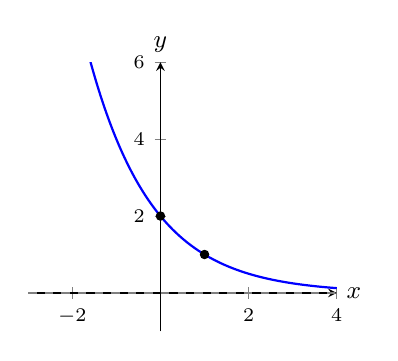
\begin{tikzpicture}
\begin{axis}[myaxis, xmin=-3,xmax=4,ymin=-1,ymax=6]
\addplot[thick,blue,domain=-2:4]{2^(1-x)};
\addplot[dashed,gray] coordinates {(-3,0)(4,0)};
\addplot[only marks,mark=*,mark size=1.5pt] coordinates {(0,2)(1,1)};
\end{axis}
\end{tikzpicture}

\textbf{(3)} $y=3^{x+1}+1$：$y=3^{x}$ を左に $1$，上に $1$ 平行移動．漸近線 $y=1$，$(0,4)$，$(-1,2)$ を通る．

\begin{tikzpicture}
\begin{axis}[myaxis, xmin=-4,xmax=2,ymin=-1,ymax=7]
\addplot[thick,blue,domain=-4:1.3]{3^(x+1)+1};
\addplot[dashed,gray] coordinates {(-4,1)(2,1)};
\addplot[only marks,mark=*,mark size=1.5pt] coordinates {(0,4)(-1,2)};
\end{axis}
\end{tikzpicture}
}

\mondai{4}{次の方程式を解け．}
\kotae{
\textbf{(1)} $4^{x-1}=8$

$2^{2(x-1)}=2^{3} \Rightarrow 2(x-1)=3 \Rightarrow x=\dfrac{5}{2}$

\textbf{(2)} $4^{x}-2^{x+1}-8=0$

$4^{x}=(2^{x})^{2}$，$2^{x+1}=2\cdot2^{x}$．$t=2^{x}>0$ とおくと
\[
t^{2}-2t-8=0 \Rightarrow (t-4)(t+2)=0
\]
$t>0$ より $t=4$，すなわち $2^{x}=2^{2}$．

$\therefore x=2$
}

\mondai{5}{次の不等式を解け．}
\kotae{
\textbf{(1)} $9^{x}<\dfrac{1}{\sqrt{3}}$

$3^{2x}<3^{-1/2}$．底 $3>1$ は単調増加：

$2x<-\dfrac{1}{2} \Rightarrow x<-\dfrac{1}{4}$

\textbf{(2)} $\left(\dfrac{1}{2}\right)^{1-3x}>\dfrac{1}{4}$

右辺 $=\left(\dfrac{1}{2}\right)^{2}$．底 $\dfrac{1}{2}<1$ は単調減少なので不等号が逆転：

$1-3x<2 \Rightarrow -3x<1 \Rightarrow x>-\dfrac{1}{3}$
}

\mondai{6}{$a>0,\;b>0$ のとき，次の式を簡単にせよ．}
\kotae{
\textbf{(1)} $\left(a^{1/2}+b^{-1/2}\right)\left(a^{1/2}-b^{-1/2}\right)$

$(A+B)(A-B)=A^{2}-B^{2}$：
\[
=a-b^{-1}=a-\dfrac{1}{b}
\]

\textbf{(2)} $\left(a^{1/4}-b^{1/4}\right)\left(a^{1/4}+b^{1/4}\right)\left(a^{1/2}+b^{1/2}\right)$

前2つの積：$a^{1/2}-b^{1/2}$．残りを掛けて
\[
(a^{1/2}-b^{1/2})(a^{1/2}+b^{1/2})=a-b
\]

\textbf{(3)} $\left(a^{1/3}-b^{1/3}\right)\left(a^{2/3}+a^{1/3}b^{1/3}+b^{2/3}\right)$

$A=a^{1/3},\;B=b^{1/3}$ とおくと $(A-B)(A^{2}+AB+B^{2})=A^{3}-B^{3}$．

$\therefore a-b$
}

\end{document}
